%
% chapter.tex -- Feldgleichungen
%
% (c) 2025 Prof Dr Andreas Müller
%
\chapter{Feldgleichungen der klassischen Physik
\label{chapter:feldgleichungen}}
\kopflinks{Feldgleichungen der klassischen Physik}

\noindent
Mit der in den letzten Kapiteln entwickelten Theorie lassen sich
die bekannten Feldgleichungen der klassischen Physik wiederfinden.
Insbesondere die Kontinuitätsgleichung, die in
Abschnitt~\ref{buch:gauss:section:erhaltungssatz}
als grundlegender erkannt wurde,
wird sich als der Kern vieler Beispiele herausstellen.

%
% Wärmeleitung und Diffusion
%
\section{Wärmeleitung und Diffusion}
\kopfrechts{Wärmeleitung und Diffunsion}
Wärmeleitung und Diffusion führen auf sehr ähnliche parabolische
partielle Differentialgleichungen.

%
% Wärmeleitung
%
\subsection{Wärmeleitung}
Die Wärmeenergiedichte $\varrho$ eines homogenenen Mediums mit der
\index{Wärmeenergiedichte}%
konstanten Wärmekapazität $c$ ist proportional zur Temperatur,
es gilt daher $\varrho=cT$.
\index{Temperatur}%
Der Wärmeleitungskoeffizient $k$ definiert, wieviel
\index{Wärmeleitungskoeffizient}%
Wärmeenergie pro Zeiteinheit den Temperaturunterschied
$\Delta T$ über eine Distanz $\Delta x$ überwindet.
In differentieller Schreibweise ist der Wärmeenergiefluss
\index{Wärmeenergiefluss}%
\[
\vec{\jmath}
=
-k \operatorname{grad} T.
\]
Da die Wärmeenergie erhalten bleibt, gilt die Kontinuitätsgleichung
\index{Kontinuitätsgleichung}%
für $\varrho$ und $\vec{\jmath}$, sie lautet
\begin{align*}
-\frac{\partial\varrho}{\partial t}
&=
\operatorname{div}\bigl(
-\kappa\operatorname{grad}T
\bigr)
\\
-c\frac{\partial T}{\partial t}
&=
-k\varrho\operatorname{div}\operatorname{grad}T
\intertext{oder nach Division durch $-c$}
\frac{\partial T}{\partial t}
&=
\kappa\,
\Delta T
\end{align*}
mit $\kappa = \frac{c}{k}$.

%
% Diffusion
%
\subsection{Diffusion}
In einem homogenen Medium ist ein Stoff mit der Konzentration 
$c$ gelöst.
\index{Konzentration}%
Konzentrationsunterschiede werden durch Diffusion des gelösten
Stoffs ausgeglichen.
\index{Diffusion}%
Je grösser der Konzentrationsunterschied, desto grösser ist
der Stofffluss, es gilt also
\[
\vec{\jmath}\, = -D\operatorname{grad}c
\]
für den Stofffluss, mit einer Materialkonstanten $D$.
\index{Stofffluss}%
Die Konzentration $c$ ist die Dichte des gelösten Stoffs,
$\vec{\jmath}$\, ist der Stofffluss im Medium.
Sofern der Stoff keine Reaktionen mit dem Medium eingeht,
bleibt die gelöste Stoffmenge erhalten, es muss daher die
Kontinuitätsgleichung
\begin{align*}
-\frac{\partial c}{\partial t}
&=
\operatorname{div}\bigl(
-D\operatorname{grad}c
\bigr)
\\
\frac{\partial c}{\partial t}
&=
D\operatorname{div}\operatorname{grad}c
\intertext{gelten.
Mit dem Laplace-Operator geschrieben ist dies}
\frac{\partial c}{\partial t}
&=
D\,\Delta c,
\end{align*}
\index{Laplace-Operator}%
eine zur Wärmeleitungsgleichung äquivalente partielle
Differentialgleichung.

%
% Fundamentallösung
%
\subsection{Fundamentallösung}
Ersetzt man die Zeitkoordinate $t$ durch $\tau=\kappa t$, wird die
Zeitableitung zu
\[
\frac{1}{\kappa}
\frac{\partial}{\partial t}
=
\frac{\partial}{\partial (\kappa t)}
=
\frac{\partial}{\partial\tau}.
\]
Durch Wahl einer geeigneten Zeiteinheit lässt sich die 
Wärmeleitungsgleichung auf $\mathbb{R}^n$ also in die Form
\begin{equation}
\frac{\partial u}{\partial t}
=
\Delta u
\label{buch:feldgleichungen:waermeleitung:eqn:normalisiert}
\end{equation}
bringen.

Die Gleichung \eqref{buch:feldgleichungen:waermeleitung:eqn:normalisiert}
hat die Fundamentallösung
\begin{equation}
u(x,t)
=
\frac{1}{(\!\sqrt{4\pi t})^{\frac{n}2}}
e^{-\frac{|x|^2}{4t}}
,
\label{buch:feldgleichungen:waermeleitung:eqn:fundamentalloesung}
\end{equation}
wie man durch Einsetzen prüfen kann.
In einer Dimension, also für $n=1$, sind die Ableitungen
\[
\left.
\begin{aligned}
\frac{\partial u}{\partial t}
&=
\frac{1}{4\!\sqrt{\pi t}}
\biggl(
\frac{x^2}{2t^2}
-
\frac{1}{t}
\biggr)
e^{-\frac{x^2}{4t}}
\\
\frac{\partial u}{\partial x}
&=
-
\frac{1}{4\!\sqrt{\pi t}} \frac{x}{t} e^{-\frac{x^2}{4t}}
&&\Rightarrow&
\frac{\partial^2 u}{\partial x^2}
&=
\frac{1}{4\!\sqrt{\pi t}}
\biggl(
\frac{x^2}{2t^2}
-\frac{1}{t}
\biggr)
e^{-\frac{x^2}{4t}}
\end{aligned}
\right\}
\quad
\Rightarrow
\quad
\frac{\partial u}{\partial t}=\Delta u.
\]
Die Wärmeleitungsgleichung ist also in diesem Fall erfüllt.

Für $n>1$ muss $\operatorname{grad}u$ und davon die Divergenz
berechnet werden.
Dies wird einfacher, wenn man beachtet, dass
\[
u(x,t)
=
u_0(x^1,t)
\dots
u_0(x^2,t)
\]
ist, wobei $u_0(x,t)$, die eindimensionale Fundamentallösung
von \eqref{buch:feldgleichungen:waermeleitung:eqn:fundamentalloesung}
ist.
Die Zeitableitung von $u(x,t)$ ist nach der Produktregel
\[
\frac{\partial u}{\partial t}(x,t)
=
\sum_{i=1}^n
u_0(x^1,t)\cdots u_0(x^{i-1})
\cdot
\frac{\partial u_0}{\partial t}(x^i,t)
\cdot
u_0(x^{i+1},t)\cdots u_0(x^n).
\]
Der Gradient $\operatorname{grad}u$ hat die Komponenten
\[
\frac{\partial u}{\partial x^i}
=
\frac{\partial}{\partial x^i}
\prod_{k=1}^n
u_0(x^k,t)
=
u_0(x^1,t)\cdots u_0(x^{i-1},t)
\cdot
\frac{\partial u_0}{\partial x}(x^i,t)
\cdot
u_0(x^{i+1},t) \cdots u_0(x^n,t).
\]
Daraus kann man die Divergenz berechnen als
\begin{align*}
\Delta u(x,t)
=
\operatorname{div}
\operatorname{grad}
u(x,t)
&=
\sum_{i=1}^n
u_0(x^1,t)\cdots u_0(x^{i-1},t)
\cdot
\frac{\partial^2 u_0}{\partial x^2}(x^i,t)
\cdot
u_0(x^{i+1},t) \cdots u_0(x^n,t).
\end{align*}
Die Differenz ist
\begin{align*}
\frac{\partial u}{\partial t}
-
\Delta u
&=
\sum_{i=1}^n
u_0(x^1,t)\cdots u_0(x^{i-1},t)
\cdot
\biggl(
\underbrace{
\frac{\partial u_0}{\partial t}(x^i,t)
-
\frac{\partial^2 u_0}{\partial x^2}(x^i,t)
}_{\displaystyle = 0}
\biggr)
\cdot
u_0(x^{i+1},t) \cdots u_0(x^n,t)
\\
&=
0.
\end{align*}
Damit ist gezeigt, dass $u(x,t)$ eine Lösung der Wärmeleitungsgleichung
ist.

Die Funktion $u_0(x,t)$ ist die Normalerteilung mit der Varianz $2t$ und
$u(x,t)$ ist eine $n$-dimensionale Normalverteilung.
Dies deckt sich mit den Erwartungen, die sich aus dem zentralen
Grenzwertsatz ergeben.
Die Diffusion von Molekülen ist setzt sich aus sehr vielen sehr
kleinen, zufälligen Stössen zusammen.
Der zentrale Grenzwertsatz sagt unter diesen Voraussetzungen eine
Normalverteilung voraus.

%
% Wellengleichung
%
\section{Wellengleichung}
\kopfrechts{Wellengleichung}
Die Wellengleichung beschreibt die Fortpflanzung einer Welle
in einem elastischen Medium.
\index{Wellengleichung}%
In diesem Abschnitt wird die Wellengleichung im eindimensionalen
Fall hergeleitet.
Es stellt sich heraus, dass man sie als die Kontinuitätsgleichung
für die Impulsdichte und den Impulsstrom verstehen kann.

%
% Die Bewegung einer Saite
%
\subsection{Die Bewegung einer Saite}
%
% fig-saite.tex
%
% (c) 2025 Prof Dr Andreas Müller
%
\begin{figure}
\centering
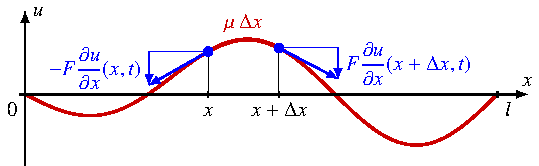
\includegraphics{chapters/080-feldgleichungen/images/saite.pdf}
\caption{Herleitung der eindimensionalen Wellengleichung für eine
schwingende Saite.
Auf das Segment der Masse $\mu\,\Delta x$ zwischen den Punkten $x$ und
$\Delta x$ wirkt eine resultierende Querkraft, die aus den blauen
Vektoren berechnet werden kann.
\label{buch:feldgleichungen:wellengleichung:fig:saite}}
\end{figure}
%
Wir betrachten eine Saite mit der linearen Massedichte $\mu$, die
zwischen den Punkten $0$ und $l$ entlang einer Geraden eingespannt
ist.
Die Spannung der Saite entlang der Geraden ist die Kraft $F$.
\index{Spannung}%
Die Funktion
\[
u
\colon
[0,l]\times \mathbb{R}
\to
\mathbb{R}
:
(x,t)
\mapsto
u(x,t)
\]
beschreibt die Auslenkung der Saite aus der Ruhelage in Abhängigkeit
von Position $x\in[0,l]|$ und der Zeit $t$.
\index{Auslenkung}%
\index{Ruhelage}%

Wir betrachten jetzt in kurzes Segment der Länge $\Delta x$ der Saite
zwischen den Koordinaten $x$ und $x+\Delta x$.
Die Masse dieses Segmentes ist $\mu \Delta x$.
Die Spannung der Saite übt eine Kraft auf das Segment aus.
Die Komponente in $x$-Richtung verschwindet.
Die Komponenten senkrecht zur Achse an den beiden 
Enden des Segmentes sind
\[
-F\frac{\partial u}{\partial x}(x,t)
\qquad\text{und}\qquad
F\frac{\partial u}{\partial x}(x+\Delta x,t),
\]
es wirkt also die gesamte Kraft
\[
F
\biggl(
\frac{\partial u}{\partial x}(x+\Delta x,t)
-
\frac{\partial u}{\partial x}(x,t)
\biggr).
\]
Das newtonsche Gesetz $F=ma$ besagt dann, dass
\index{newtonsches Gesetz}%
\[
F
\biggl(
\frac{\partial u}{\partial x}(x+\Delta x,t)
-
\frac{\partial u}{\partial x}(x,t)
\biggr)
=
\mu\Delta x\cdot \frac{\partial^2 u}{\partial t^2}(x,t).
\]
Division durch $\Delta x$ und der Grenzübergang $\Delta x\to 0$ ergibt
auf der linken Seite eine zweite Ableitung
\[
F
\frac{\partial^2u}{\partial x^2}(x,t)
=
\mu
\frac{\partial^2u}{\partial t^2}(x,t).
\]
Nach Division durch $\mu$ entsteht die eindimensionale Wellengleichung
\index{Wellengleichung!eindimensional}%
\begin{equation}
\frac{\partial^2 u}{\partial t^2}
=
a^2
\frac{\partial^2 u}{\partial x^2}
\qquad\text{mit}\quad
a^2=\displaystyle\frac{F}{\mu},
\label{buch:feldgleichungen:wellengleichung:eqn:wellengleichung}
\end{equation}
wobei $a$ die Ausbreitungsgeschwindigkeit einer Welle entlang der
Saite ist.
Die Geschwindigkeit wird geringer, wenn die Massedichte grösser wird,
sie wird grösser, wenn die Spannung der Saite steigt.

%
% Impulsdichte und Impulsstrom
%
\subsection{Impulsdichte und Impulsstrom}
Der Ausdruck
\[
\mu \,\Delta x \,\frac{\partial u}{\partial t}(x,t)
\]
ist der Impuls eines Segmentes der Länge $\Delta x$ der Saite
an der Stelle $x$ zur Zeit $t$.
Somit ist
\[
\varrho(x,t)
=
\mu\frac{\partial u}{\partial t}(t,x)
\]
die Impulsdichte der Saite.
\index{Impulsdichte}%
Da der Impuls erhalten ist, suggeriert dies, dass die Wellengleichung
die Kontinuitätsgleichung für Impulsdichte und Impulsstrom ist.

Die Spannung der Saite führt wie in der Herleitung der Wellengleichung
ausgeführt zu einer Kraft quer zur Saite.
Zwischen den Punkten $x$ und $\Delta x$ besteht der Auslenkungsunterschied 
\[
u(x+\Delta x, t) - u(x,t)),
\]
was zu einer Kraft
\[
F \frac{u(x+\Delta x, t) - u(x,t)}{\Delta x}
\]
führt.
Die Kraft bewirkt eine Reduktion des Impulses am rechten Ende des
Segmentes, und eine Zunahme am linken Ende.
Es kommt also zu einem Fluss der Impulsdichte vom rechten zum linken
Ende.
Wir erkennen, dass
\[
\vec{\jmath}
=
-F
\operatorname{grad} u(x,t)
\]
der Impulsstrom der Saite ist.
\index{Impulsstrom}%
Da der Impuls erhalten ist, gilt die Kontinuitätsgleichung
\begin{align*}
-\frac{\partial \varrho}{\partial t}(x,t)
&=
\operatorname{div}
\bigl(
-F\operatorname{grad} u(x,t)
\bigr)
\\
-\mu
\frac{\partial^2 u}{\partial t^2}
&=
-F \operatorname{div}\operatorname{grad} u
\intertext{oder nach Division durch $-\mu$}
\frac{\partial^2 u}{\partial t^2}
&=
\frac{F}{\mu}
\Delta u.
\end{align*}
Die Wellengleichung ist also die Kontinuitätsgleichung für den
Impulsstrom.


%
% Lösungsverfahren für partielle Differentialgleichungen
%
\section{Lösungsverfahren für lineare partielle Differentialgleichungen}
\kopfrechts{Lösungsverfahren}
Die Wärmeleitungs-, Diffunsions- und Wellengleichungen sind Beispiele
von linearen partiellen Differentialgleichungen.
Die Lösung solcher Gleichungen ist ein eigenes mathematisches
Fachgebiet, hier können daher nur einige wenige Hinweise auf die
grundlegenden Lösungsverfahren gegeben werden.

%
% definitionsgebiet und Randbedingungen
%
\subsection{Definitionsgebiet und Randbedingungen}
%
% fig-gebiet.tex
%
% (c) 2025 Prof Dr Andreas Müller
%
\begin{figure}
\centering
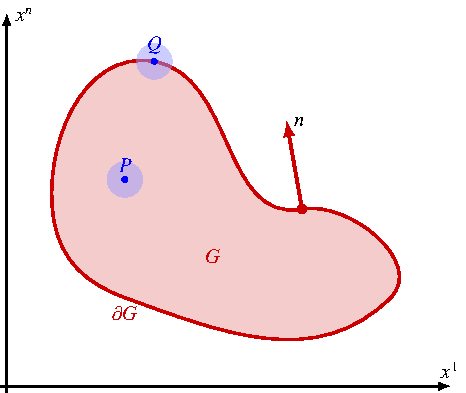
\includegraphics{chapters/080-feldgleichungen/images/gebiet.pdf}
\caption{Gebiet und Rand.
Der Punkt $P$ ist ein innerer Punkt des Gebietes, da es eine kleine
Umgebung gibt, die vollständig in $G$ enthalten ist.
Der Punkt $Q$ ist ein Randpunkt, $Q\in\partial G$, weil jede Umgebung
sowohl Punkte von $G$ wie auch von $\mathbb{R}^n\setminus G$ enthält.
Die Normale $n$ auf den Rand wird zur Definition der Neumann-Randbedingungen
verwendet.
\label{buch:feldgleichungen:loesungsverfahren:fig:gebiet}}
\end{figure}
%
Die Lösung einer partiellen Differentialgleichung ist erst dann vollständig
bestimmt, wenn zusätzlich zur Gleichung geeignete Randbedingungen
vorgegeben werden.

%
% Definitionsgebiet
%
\subsubsection{Definitionsgebiet}
Das Definitionsgebiet kann eine beliebige offene Menge $G\subset\mathbb{R}^n$
sein.
Zur Berechnung partieller Ableitungen einer Funktion in einem Punkt
muss man Funktionswerte in jeder beliebigen Richtung ausgehend von
diesem Punkt auswerten können.
Dies ist nur möglich, wenn es um jeden Punkt von $G$ auch eine kleine
Umgebung gibt, die ebenfalls im Definitionsgebiet der Funktion enthalten
ist.
In Abbildung~\ref{buch:feldgleichungen:loesungsverfahren:fig:gebiet}
ist $P$ ein innerer Punkt des Gebietes $G$.
Nur für solche inneren Punkte ist es sinnvoll zu sagen, dass eine
Funktion die Differentialgleichung erfüllt.

Randbedingungen müssen auf Randpunkten des Gebietes spezifiziert werden.
Dies sind Punkte $x\in\mathbb{R}^n$, für die jede kleine Umgebung sowohl
Punkte von $G$ wie auch ausserhalb von $G$ enthält.
In Abbildung~\ref{buch:feldgleichungen:loesungsverfahren:fig:gebiet}
ist $Q$ ein Randpunkt.
Die Menge der Randpunkte von $G$ wird mit $\partial G$ bezeichnet.
Die Menge $\bar{G}=G\cup \partial G$ enthält sowohl das Gebiet
wie auch die Randpunkte.

Eine Lösung der Differentialgleichung ist eine stetige Funktion
$u\colon\bar{G}\to\mathbb{R}$, die im Inneren, also auf $G$,
genügend oft stetig differenzierbar ist und
die Differentialgleichung erfüllt.
Ausserdem müssen auf einem Teil der Randpunkte zusätzlich
Randbedingungen erfüllt sein.
Da $u$ auch auf dem Rand $\partial G\subset\bar{G}$ definiert
ist, können diese ebenfalls verifiziert werden.

%
% Dirichlet-Randbedingungen
%
\subsubsection{Dirichlet-Randbedingungen}
\index{Dirichlet-Randbedingungen}%
{\em Dirichlet-Randbedingungen} geben Wert der Funktion vor.
Sei also $D\subset\partial G$ eine Teilmenge der Randpunkte
und $g\colon D\to\mathbb{R}$ eine Funktion, dann erfüllt $u$
die Dirichlet-Randbedingung mit den Randwerten $g$, wenn
\[
u(x) = g(x)\qquad \forall x\in D
\]
gilt.

Dirichlet-Randbedingungen liegen im Beispiel der schwingenden Saite
an den Punkten $x=0$ und $x=l$ vor.
Dort sind die Funktionswerte $0$ vorgeben.
Solche Randbedingungen mit Wert 0 werden auch {\em homogenen} 
Randbedingungen genannt.

Die Anfangslage $u(x,0)$ der schwingenden Saite war dagegeben durch
die Funktion $f(x)$ vorgegeben, dies sind Dirichlet-Randbedingungen
auf der Menge $\{(x,0)\mid x\in[0,l]\}$.

\subsubsection{Neumann-Randbedingungen}
\index{Neumann-Randbedingungen}%
{\em Neumann-Randbedingungen} geben statt Funktionswerten die Werte
von Ableitungen vor.
Solche Randwerte können im Allgmeinen die Lösung nicht eindeutig
festlegen, es muss mindestens ein Funktionswert ebenfalls vorgegeben
werden.
Aus einem Funktionswert auf dem Rand und der Ableitung entlang
der Randkurve können durch Integration die Werte auf der Randkurve
ermittelt werden, so dass tatsächlich Dirichlet-Randbedingungen
vorliegen.

Nur Ableitungen senkrecht auf den Rand können tatsächlich neue
Information liefern, die nicht auch durch Dirichlet-Randbedingungen
vorgegeben werden können.
Bezeichnet man mit $n$ die Normale auf den Rand des Gebietes
(Abbildung~\ref{buch:feldgleichungen:loesungsverfahren:fig:gebiet}),
dann wird die Ableitung senkrecht auf den Rand mit
\[
\frac{\partial u}{\partial n}
=
D_n u
\]
bezeichnet und heisst die {\em Normalableitung}.
\index{Normalableitung}%
Neumann-Randbedingungen geben auf einer Teilmenge $N\subset\partial G$
die Normalableitung vor.

Neumann-Randbedingungen lagen im Beispiel der schwingenden Saite bei
der Vorgabe der Anfansgeschwindigkeit
\[
\frac{\partial u}{\partial t}(x,0)
=
g(x)
\]
vor.
Die Ableitung in Richtung $t$ ist die Normalableitung auf dem Randstück
$[0,l]\times \{0\}$ des Randes.

\subsection{Separationsverfahren}
\index{Separationsverfahren}%
Das Verfahren wird am Beispiel der Wellengleichung
\eqref{buch:feldgleichungen:wellengleichung:eqn:wellengleichung}
in der eindimensionalen Form
\begin{equation}
\frac{\partial^2 u}{\partial t^2}
=
a^2
\frac{\partial^2 u}{\partial x^2}
\label{buch:feldgleichungen:loesung:eqn:wellengleichung}
\end{equation}
illustriert.
Es funktioniert, wenn das Gebiet $G$ auf dem die Funktion $u$
definiert ist, ein Rechteck ist.
Für den vorliegenden Fall nehmen wir an, dass $u$ auf
$[0,l]\times\mathbb{R}$ definiert ist, und dass an den
Intervall-Enden homogene Dirichlet-Randbedingungen der Form 
\[
u(0,t)=u(l,t)=0
\]
gegeben sind.
Neumann-Randbedingungen können auf analoge Art behandelt werden.

Wir nehmen an, dass sich die Lösung als Produkt $u(x,t)=X(x)T(t)$
von zwei Funktionen schreiben, wobei $X$ nur von $x$ und $T$ nur
von $t$ abhängt.
Durch Einsetzen des Ansatzes in
\eqref{buch:feldgleichungen:loesung:eqn:wellengleichung} 
ist
\[
T''(t) X(x)
=
a^2
T(t)
X''(x).
\]
Nach Division durch $u$ lassen sich die nicht abgeleiteten Faktoren
kürzen und es bleibt
\begin{equation}
\frac{T''(t)}{T(t)}
=
a^2
\frac{X''(x)}{X(x)}.
\label{buch:feldgleichungen:loesung:eqn:separiert}
\end{equation}
Die linke Seite hängt nur von $t$ ab, während die rechte nur von $x$
abhängt.
Man sagt, die Variablen sind {\em separiert} worden.
Die Gleichung~\eqref{buch:feldgleichungen:loesung:eqn:separiert}
kann nur erfüllt werden, wenn beide Seiten konstant sind.
Es gibt daher eine Konstante $\lambda$, mit der sich die
Gleichung~\eqref{buch:feldgleichungen:loesung:eqn:separiert}
in die zwei Gleichungen
\[
\begin{aligned}
\frac{T''(t)}{T(t)}&=\lambda &&\Rightarrow& T''(t) &= \lambda T(t) \\
\frac{X''(x)}{X(x)}&=\lambda &&\Rightarrow& X''(x) &= \lambda X(x)
\end{aligned}
\]
zerlegen lässt.
Dies sind gewöhnliche Differentialgleichungen, die sich unabhängig
voneinander lösen lassen.

Für $\lambda > 0$ wachsen die Lösungen exponentiell schnell an, was
nicht dem Verhalten einer Welle entspricht.
Wir dürfen daher annehmen, dass $\lambda \le 0$ ist und schreiben
$\lambda = -k^2$ mit $k\in\mathbb{R}$, um dies sicherzustellen.
Die Differentialgleichungen bekommen daher die Form
\begin{align*}
X''(x) &= -k^2 X(x)
&&\text{und}&
T''(t) &= -k^2 T(t),
\intertext{die die Lösungen}
X(x) &= A\cos kx + B \sin kx
&&\text{und}&
T(t) &= A\cos kt + B \sin kt
\end{align*}
haben.

Für die Bestimmung der Koeffizienten $A$ und $B$ müssen die 
Randbedingungen hinzugezogen werden.
Dies können nicht für jeden Wert von $k$ erfüllt werden.
Die homogenen Randbedingungen für $X(x)$ verlangen, dass
\begin{equation*}
\left.
\bgroup
\renewcommand{\arraycolsep}{1pt}
\begin{array}{rlcrlcl}
A&\cos 0 &\,+\,&B&\sin 0  &\,=\,& 0\\
A&\cos kl&\,+\,&B&\sin kl &\,=\,& 0
\end{array}
\egroup
\quad
\right\}
\qquad\Rightarrow\qquad
\left\{
\quad
\begin{aligned}
        A&= 0 \\
B\sin kl &= 0.
\end{aligned}
\right.
\end{equation*}
Da $B=0$ nur die Null-Lösung ergäbe, muss $\sin kl=0$ sein, was nur
dann möglich ist, wenn $kl$ ein Vielfaches von $\pi$ ist.
Es gibt also eine natürliche Zahl $n$ derart, dass
$kl=n\pi$ und daher $k=n\pi/l$.
Die Randbedingungen legen daher fest, dass für jedes natürlich $n$ eine
Lösung
\[
X(x) = B \sin \frac{n\pi x}{l}
\qquad\text{und}\qquad
T(t) = A \cos \frac{n\pi t}{l} + B \sin\frac{n\pi t}{l}
\]
gefunden werden kann.

Dank der Linearität der Gleichung kann die allgemeine Lösung der
Wellengleichung jetzt durch die Überlagerung
\[
u(x,t)
=
\sum_{n=1}^\infty
\biggl(
a_n\cos\frac{n\pi t}{l}
+
b_n\sin\frac{n\pi t}{l}
\biggr)
\sin\frac{n\pi x}{l}
\]
konstruiert werden, deren Koeffizienten $a_n$ und $b_n$ durch
Heranziehen weitere Randbedingungen bestimmt werden müssen.

Seien jetzt zusätzlich Dirichlet- und Neumann-Randbedingungen zur Zeit
$t$ gegeben.
Es gibt daher Funktionen $f(x)$ und $g(x)$, die
\[
\renewcommand{\arraycolsep}{2pt}
\begin{array}{rclcl}
u(x,0)
&=&
\displaystyle
\sum_{n=0}^\infty \phantom{\frac{n\pi}{l}}a_n \sin\frac{n\pi x}{l}
&=&
f(x) \\
\displaystyle
\frac{\partial u}{\partial t}(x,0)
&=&
\displaystyle
\sum_{n=0}^\infty \frac{n\pi}{l}b_n \sin\frac{n\pi x}{l}
&=&
g(x).
\end{array}
\]
Zur Bestimmung der Koeffizienten $a_n$ und $b_n$ müssen wir die
Funktionen $f$ und $g$ in eine Fourier-Sinusreihe
\begin{align*}
f(x) & = \sum_{n=1}^\infty b_n(f)\sin \frac{n\pi x}{l} \\
g(x) & = \sum_{n=1}^\infty b_n(g)\sin \frac{n\pi x}{l}
\end{align*}
entwickeln.
Dann können die Koeffizienten durch Koeffizientenvergleich gefunden
werden.
Die Lösung ist dann
\[
u(x,t)
=
\sum_{n=1}^\infty
\biggl(
b_n(f)
\cos\frac{n\pi t}{l}
+
\frac{lb_n(g)}{n\pi}
\sin\frac{n\pi t}{l}
\biggr)
\sin\frac{n\pi x}{l}.
\]

\subsection{Transformationsverfahren}
\index{Transformationsverfahren}%
Die Lösung der Wellengleichung mit dem Separationsverfahren hat 
auf ganz natürlich Art und Weise auf Fourier-Reihen geführt.
So hat auch Joseph Fourier im 19.~Jahrhundert die nach ihm benannten
Reihen entdeckt.
Es liegt daher nahe zu vermuten, dass sich partielle Differentialgleichungen
auch lösen lassen, indem man sie einer Integraltransformation
unterwirft.
Wir illustrieren dies am Beispiel der Wärmeleitung in einem 
an den Enden isolierten Stab.

Wir betrachten die Differentialgleichung
\[
\frac{\partial T}{\partial x}
=
\kappa
\frac{\partial^2 T}{\partial x^2}
\]
auf dem Gebiet $[0,\pi]\times\mathbb{R}^+$, wobei wir das Intervall
vor allem deshalb gewählt haben, weil sich damit später einfachere
Formeln ergeben.
Ausserdem werden homogene Neumann-Randbedingungen an den
Intervallenden angenommen.
Dies bedeutet, dass die Ableitungen nach $x$ an den Intervallenden
verschwinden, was physikalisch bedeutet, dass kein Wärmeaustausch
über die Enden des Stabes erfolgt.
Ausserdem wird die Temperaturverteilung $T(x)=T(x,0)$ zur Zeit $t=0$
vorgegeben.

Da die Ableitung von $u$ nach $x$ für $x=0$ und $x=\pi$ verschwinden
muss, kann man die Funktion $x\mapsto u(x,t)$ zu einer in $x$
geraden Funktion auf dem Intervall $[-\pi,\pi]$ ausdehnen, die
man ihrerseits zu einer $2\pi$-periodischen Funktion erweitern kann.
Somit muss es eine Entwicklung der Funktion $T(x,t)$ in
eine Fourier-Kosinusreihe
\[
T(x,t)
=
\frac{a_0(t)}{2}
+
\sum_{n=1}^\infty
a_n(t) \cos nx
\]
geben.
Setzt man sie in die Wärmeleitungsgleichung ein, erhält man
\[
\frac{\dot{a}_0}{2}
+
\sum_{n=1}^\infty
\dot{a}_n(t) \cos nx
=
-
\kappa
\sum_{n=1}^\infty
n^2
\cos nx.
\]
Durch Koeffizientenvergleich findet man die gewöhnlichen
Differentialgleichungen
\begin{align}
\dot{a}_0(t)&=0
&&\text{und}&
\dot{a}_n(t)&=-n^2 a_n(t).
\label{buch:feldgleichungen:loesungen:transformation:ode}
\end{align}
Zur Lösung dieser Differentialgleichungen werden zusätzlich
Anfangsbedingungen benötigt, die man aus der Entwicklung der
Funktion $T(x)$ in eine Fourier-Kosinusreihe gewinnen kann.
\index{Fourier-Kosinusreihe}%
Aus 
\[
T(x)
=
\frac{A_0}2
+
\sum_{n=1}^\infty A_n \cos nx
\]
kann man ablesen, dass
\begin{align*}
a_0(0) &= A_0
&&\text{und}&
a_n(0) &= A_n
\end{align*}
sein muss.
Damit kann man jetzt die Lösung der Differentialgleichungen
\eqref{buch:feldgleichungen:loesungen:transformation:ode}
finden.
Die erste Differentialgleichung sagt, dass $a_0(t)=A_0$ konstant ist.
Die zweite Differentialgleichung sagt, dass $a_n(t) = A_ne^{-n^2t}$
sein muss.
Daraus lässt sich die Lösung als
\[
T(x,t)
=
\frac{A_0}{2}
+
\sum_{n=1}^\infty
A_n
e^{-n^2t}
\cos nx
\]
zusammensetzen.


%
% Feldgleichunge, die sich durch zusätzliche Annahmen ergeben
%
\section{Feldgleichungen, die sich durch zusätzliche Annahmen ergeben}
\kopfrechts{Zusätzliche Annahmen}
Oft lassen sich Feldgleichungen mit Hilfe zusätzlicher Annahmen
vereinfachen.
Eine stationäre Lösung einer partiellen Differentialgleichung ist
eine Lösung, die nicht von der Zeit abhängt, in der also alle
Zeitableitungen verschwinden.

\subsection{Die Poisson-Gleichung}
In der Elektrostatik sind die Ladungen, die das elektrostatische
Feld erzeugen, unbeweglich, und das Feld ändert sich mit der Zeit
nicht.
Aus den Maxwell-Gleichungen, die in Kapitel~\ref{chapter:maxwell}
ausführlicher diskutiert werden, folgt dann, dass das elektrische
Feld ein Potentialfeld ist und dass das Potential $\varphi$ die
Differentialgleichung
\begin{equation}
\Delta \varphi = 4\pi \varrho
\label{buch:feldgleichungen:zusätzlich:eqn:poisson}
\end{equation}
erfüllt, wobei $\varrho$ die Ladungsdichte ist.
Die Gleichung~\eqref{buch:feldgleichungen:zusätzlich:eqn:poisson}
heisst auch die {\em Poisson-Glei\-chung}.
\index{Poisson-Gleichung}%
Sie tritt zum Beispiel auch bei Minimalflächen in linearer Näherung
auf, wenn zwischen den beiden Seiten der Fläche ein Druckunterschied
vorliegt.

\subsection{Die Laplace-Gleichung}
Aus der Poisson-Gleichung \eqref{buch:feldgleichungen:zusätzlich:eqn:poisson}
ergibt sich im Vakuum, wo keine Ladungen vorhanden sind, die noch
einfachere Gleichung
\[
\Delta \varphi = 0,
\]
die auch die {\em Laplace-Gleichung} genannt wird.
\index{Laplace-Gleichung}%
Sie tritt auch im Grenzfall einer stationären Temperaturverteilung
auf, denn in diesem Fall verschwindet die Zeitableitung in der
Wärmeleitungsgleichung.
Die Lösungen der Laplace-Gleichung heissen auch {\em harmonische} 
Funktionen.

\subsection{Die Helmholtz-Gleichung}
Die Wellengleichung in zwei Dimension hat die Form
\[
\frac{1}{a^2}
\frac{\partial^2u}{\partial t^2}
=
\frac{\partial^2 u}{\partial x^2}
+
\frac{\partial^2 u}{\partial y^2}.
\]
Auch hier kann man einen Separationsansatz versuchen und
\[
u(x,y,t) = T(t) v(x,y)
\]
ansetzen.
Einsetzen in die Differentialgleichung ergibt
\[
\frac{1}{a^2}
T''(t) v(x,y)
=
T(t)
\biggl(
\frac{\partial^2 v}{\partial x^2}
+
\frac{\partial^2 v}{\partial y^2}
\biggr).
\]
Division durch $u$ separiert die Variablen, den in
\[
\frac{1}{a^2}
\frac{T''(t)}{T(t)}
=
\frac{\Delta v(x,y)}{v(x,y)}
\]
hängt die linke Seite nur von $t$, die rechte nur von $x$ und $y$ ab.
Beide Seiten sind daher konstant.
Wir bezeichnen die Konstante mit mit $-\lambda^2$ und bekommen die
beiden separierten Differentialgleichungen
\[
T''(t) = -a^2\lambda^2 T(t)
\qquad\text{und}\qquad
\Delta v = -\lambda^2 v.
\]
Die Differentialgleichung für $T$ ist eine gewöhnliche
Schwingungsdifferentialgleichung mit der allgemeinen Lösung
\[
T(t) = A\cos a\lambda t + B \sin a\lambda t.
\]
Es muss daher nur noch die zweite Differentialgleichung gelöst
werden.
In allgemeinster Form ist dies die Gleichung
\begin{equation}
\Delta v = \lambda v,
\end{equation}
die auch die {\em Helmholtz-Gleichung} heisst.
\index{Helmholtz-Gleichung}%


Bei der schwingenden Saite reduziert sich die Helmholtz-Gleichung
auf die Differentialgleichung
\[
X''(x) = \lambda X(x),
\]
die sich ebenfalls mit trigonometrischen Funktionen lösen lässt.
Auf einem endlichen Intervall der Länge $l$ mit Dirichlet-Randbedingungen
sind Lösungen nur für $\lambda=n\pi/l$, $n\in\mathbb{N}$ möglich.

Die allgemeine Theorie der Helmholtz-Gleichung zeigt, dass für
kompakte Gebiete mit ausreichend glattem Rand und Dirichlet-Randbedingungen
eine diskrete Folge $(\lambda_n)_{n\in\mathbb{N}}$ von möglichen Werten
für $\lambda$ mit jeweils endlichdimensionalen Lösungsraum der Dimension
$k(n)$ existiert, aus denen sich alle Lösungen
\[
u(x,t)
=
\sum_{n=0}^\infty
\sum_{k=1}^{k(n)}
\bigl(
a_n
\cos a\lambda_n t
+
b_n
\sin a\lambda_n t
\bigr)
u_{n,k}(x)
\]
zusammensetzen lassen, wobei die Funktionen $u_{n,k}$, $k=1,\dots,k(n)$
eine Basis des Lösungsraumes der Helmholtz-Gleichung für $\lambda=\lambda_n$
ist.

Auch aus der Wärmeleitungsgleichung auf dem Gebiet $G$ entsteht
mit Hilfe des obigen Separationsansatzes eine Helmholtz-Gleichung.



